  
 
  
  
\begin{frame}\frametitle{Factors flow graph} 
  
  
\begin{center} 
  
  
\begin{figure} 
  
  
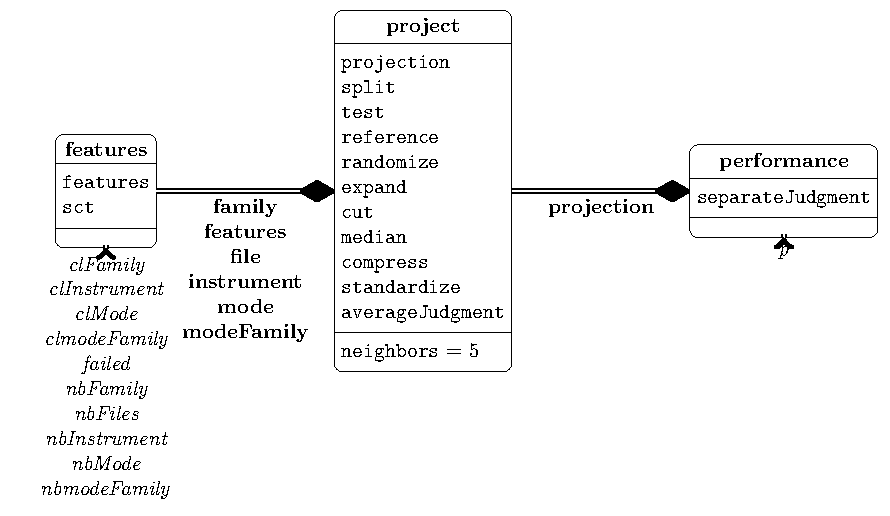
\includegraphics[width=\textwidth,height=0.8\textheight,keepaspectratio]{../figures/factors.pdf} 
  
  
\label{factorFlowGraph} 
  
  
\end{figure} 
  
  
\end{center} 
  
  
\end{frame} 
  
\begin{frame}\frametitle{consensus vs averaging} 
  
\begin{table} 
\begin{center} 
\ 
 \setlength{\tabcolsep}{.16667em} 
\begin{tabular}{lllc} 
features & separateJudgment & averageJudgment & none \\ 
\hline 
mfcc & 0 & 0 & 86.3 \\ 
mfcc & 0 & 1 & 86.5 \\ 
mfcc & 1 & 0 & 86.2 \\ 
scat & 0 & 0 & 93.3 \\ 
scat & 0 & 1 & 95.5 \\ 
scat & 1 & 0 & 98.1 \\ 
tfscat & 0 & 0 & 98.0 \\ 
tfscat & 0 & 1 & 99.0 \\ 
tfscat & 1 & 0 & 99.5 \\ 
\end{tabular} 
\end{center} 
\label{sc1000PrlmTe1RejuRa0Ex0Cu1Me1Co1St1} 
\end{table} 
 
\end{frame}  
  
\begin{frame}\frametitle{\small split: 50, test: 1, reference: judgments, randomize: 0, expand: 0, cut: 1, median: 1, compress: 1, standardize: 1} 
\begin{center} 
\begin{figure} 
\centering 
\includegraphics[width=\textwidth,height=0.8\textheight,keepaspectratio]{./figures/Fig207.pdf} 
\label{sp50Te1RejuRa0Ex0Cu1Me1Co1St1} 
\end{figure} 
\end{center} 
  
  
\end{frame}  
